% Pre-ambulo
\documentclass[a4paper, 12pt]{abnt}

%% Pacotes para texto em Inglês
% \usepackage[brazil]{babel}
% \usepackage[T1]{fontenc}
% \usepackage[latin1]{inputenc}
 
%% Pacotes para texto em Portugues
\usepackage[brazil]{babel}
\usepackage[utf8]{inputenc}
\usepackage[T1]{fontenc}
 
\usepackage{dsfont}
\usepackage{amssymb,amsmath}
\usepackage{multirow}
\usepackage[alf]{abntcite}
\usepackage[pdftex]{color, graphicx}
\usepackage{colortbl} 
\usepackage{url}
\usepackage{abnt-alf}
\usepackage{abntcite}
\usepackage{algorithm}
\usepackage{algorithmic}
%\usepackage{alg} 
%\usepackage{hyperref}
\usepackage{framed}


% Redefinicao de instrucoes
\floatname{algorithm}{Algoritmo}
\renewcommand{\algorithmicrequire}{\textbf{Entrada:}}
\renewcommand{\algorithmicensure}{\textbf{Saída:}}
\renewcommand{\algorithmicend}{\textbf{fim}}
\renewcommand{\algorithmicif}{\textbf{se}}
\renewcommand{\algorithmicthen}{\textbf{então}}
\renewcommand{\algorithmicelse}{\textbf{senão}}
\renewcommand{\algorithmicfor}{\textbf{para}}
\renewcommand{\algorithmicforall}{\textbf{para todo}}
\renewcommand{\algorithmicdo}{\textbf{faça}}
\renewcommand{\algorithmicwhile}{\textbf{enquanto}}
\renewcommand{\algorithmicloop}{\textbf{loop}}
\renewcommand{\algorithmicrepeat}{\textbf{repetir}}
\renewcommand{\algorithmicuntil}{\textbf{até que}}
\renewcommand{\algorithmiccomment}[1]{\% #1}

\newcommand{\writeauthor}{Jamillo G. da S. Santos}
\newcommand{\writeteacher}{Prof. Dr. Eduardo Braulio}
\newcommand{\writeteacheren}{Prof. Doc. Eduardo Braulio}
\newcommand{\writedate}{Abril 2017}

\newenvironment{guide}{%
	\color{red}
	\vspace{5mm}
	{\LARGE GUIA:}
	\hrule
}{
	\vspace{1.5mm}
	\hrule
	\vspace{5mm}
}%


% Definicao da lista de simbolos
% \simb[entrada na lista de simbolos]{simbolo}:
% Escreve o simbolo no texto e uma entrada na lista de simbolos.
% Se o parametro opcional e omitido, usa-se o parametro obrigatorio.
\newcommand{\simb}[2][]
{%
	\ifthenelse{\equal{#1}{}}
	{\addcontentsline{los}{simbolo}{#2}}
	{\addcontentsline{los}{simbolo}{#1}}#2
}
% Para aceitar comandos com @ (at) no nome
\makeatletter 
% \listadesimbolos: comando que imprime a lista de simbolos
\newcommand{\listadesimbolos}
{
	\pretextualchapter{Lista de símbolos}
	{\setlength{\parindent}{0cm}
	\@starttoc{los}}
}
% Como a entrada sera impressa
\newcommand\l@simbolo[2]{\par #1}
\makeatother


% Definicao da lista de abreviaturas e siglas
% \abrv[entrada na lista de simbolos]{abreviatura}:
% Escreve a sigla/abreviatura no texto e uma entrada na lista de abreviaturas e siglas.
% Se o parametro opcional e omitido, usa-se o parametro obrigatorio.
\newcommand{\abrv}[2][]
{%
	\ifthenelse{\equal{#1}{}}
	{\addcontentsline{loab}{abreviatura}{#2}}
	{\addcontentsline{loab}{abreviatura}{#1}}#2
}
% Para aceitar comandos com @ (at) no nome
\makeatletter 
% \listadeabreviaturas: comando que imprime a lista de abreviaturas e siglas
\newcommand{\listadeabreviaturas}
{
	\pretextualchapter{Lista de abreviaturas e siglas}
	{\setlength{\parindent}{0cm}
	\@starttoc{loab}}
}
% Como a entrada sera impressa
\newcommand\l@abreviatura[2]{\par #1}
\makeatother


% \listofalgorithms: comando que imprime a lista de algoritmos
\renewcommand{\listalgorithmname}{Lista de algoritmos}


% Hifeniza������o de palavras feita de forma incorreta pelo LaTeX
\hyphenation{PYTHON ou-tros}


% Inicio do documento
\begin{document}

	\frenchspacing
	
	% Capa (arquivo Includes/Capa.tex)
	% Capa
% Prote��o externa do trabalho e sobre a qual se imprimem as informa��es indispens�veis 
% � sua identifica��o.

% Especifica��o da capa
\begin{titlepage}
	\begin{center}
		
		  
		\begin{minipage}{11.15cm}
			\begin{center}
				\begin{espacosimples}
					{\small \ \\
                       \textsc{Instituto Federal do Rio Grande do Norte}
                       \\
							  \textsc{Campus Natal - Central}					\\
							  \textsc{Diretoria de Gestão e Tecnologia da Informação}	   
							  \\
							  \textsc{Tecnologia em Análise e Desenvolvimento de Sistemas}}   	
                       \\
				\end{espacosimples}
			\end{center}
		\end{minipage}

			
		\vspace{6cm}
						
		% T�tulo do trabalho
		{\setlength{\baselineskip}%
		{1.3\baselineskip}
		{\LARGE \textbf{Título do trabalho}}\par}
			
		\vspace{3cm}
			
		% Nome do aluno (autor)
		{\large \textbf{Jamillo G. da S. Santos}}
						
		\vspace{6cm}
		
		% Local da institui��o onde o trabalho deve ser apresentado e ano de entrega do mesmo
		Natal-RN\\Abril 2017
	\end{center}
\end{titlepage}

	% Folha de rosto (arquivo extra-includes/FolhaRosto.tex)
	% Folha de rosto
% Cont�m os elementos essenciais � identificação do trabalho.

% T�tulo, nome do aluno e respectivo orientador e filiação
\titulo{\Large{Título}}
\autor{Nome completo do autor}
\orientador[Orientador]{\par Nome completo do orientador e titulação}
\instituicao
{
   TADS -- Curso de Tecnologia em Análise e Desenvolvimento de
   Sistemas\par 
   DIATINF -- Diretoria Acadêmica de gestão e Tecnologia da Informação\par 
   CNAT -- Campus Natal - Central\par 
   IFRN -- Instituto Federal do Rio Grande do Norte }
	
% Natureza do trabalho (não deve ser modificada)
\comentario
{
	Trabalho de conclusão de curso de graduação do curso de Tecnologia e Análise em
	Desenvolvimento de Sistemas da Diretoria de Gestão e Tecnologia de Informação
	do Instituto Federal do Rio Grande do Norte como requisito parcial para a
	obtenção do grau de Tecnologo em Análise e Desenvolvimento de
	Sistemas.\bigskip\\
   \textit{Linha de pesquisa}:\\Nome da linha de pesquisa
}
		
% Local e data
\local{Natal-RN}
\data{Mês e ano}
	
\folhaderosto	
	
	% Folha de aprovacao (arquivo extra-includes/FolhaAprovacao.tex)
	% Folha de aprova��o
\begin{folhadeaprovacao}
	\setlength{\ABNTsignthickness}{0.4pt}
	\setlength{\ABNTsignwidth}{10cm}
	
	\noindent 
	Trabalho de Conclusão de Curso de Graduação sob o título
	\textit{Título} apresentada por Nome completo do autor e aceita pelo Diretoria
	de Gestão e Tecnologia da Informação do Instituto Federal do Rio Grande do
	Norte, sendo aprovada por todos os membros da banca examinadora abaixo especificada:
		
	% Membros da banca examinadora e respectivas filia��es
	\assinatura
	{
		Nome completo do orientador e titulação   			                  \\
		{\small Presidente}											          \smallskip\\ 
		{\footnotesize
			DIATINF -- Diretoria Acadêmica de Gestão e Tecnologia da Informação		   \\
		  	IFRN -- Instituto Federal do Rio Grande do Norte
		}
   }
      
   \assinatura
	{
      Nome completo do examinador e titulação   			                  \\
		{\small Examinador}											          \smallskip\\ 
		{\footnotesize
			Diretoria/Departamento		\\
		  	Instituto
		}
   }   
   
   \assinatura
	{
      Nome completo do examinador e titulação   			                  \\
		{\small Examinador}											          \smallskip\\ 
		{\footnotesize
			Diretoria/Departamento		\\
		  	Universidade
		}
	}
		
	\vfill
	
	\begin{center}
		Natal-RN, data da defesa (dia, mês e ano).
	\end{center}
\end{folhadeaprovacao}
	
	
	% Dedicatoria (arquivo extra-includes/Dedicatoria.tex)
	% Dedicat�ria

\chapter*{}
\vspace{15cm}
\begin{flushright}
	Homenagem que o autor presta a uma ou mais pessoas.
\end{flushright}
	
	% Agradecimentos (arquivo extra-includes/Agradecimentos.tex)
	% Agradecimentos

\chapter*{Agradecimentos}

Agradecimentos dirigidos àqueles que contribuíram de maneira relevante à
elaboração do trabalho, sejam eles pessoas ou mesmo organizações.

   
   % Epigrafe (arquivo extra-includes/Epigrafe.tex)
	% Ep�grafe (cita��o seguida de indica��o de autoria)

\chapter*{}
\vspace{15cm}
\begin{flushright}

\textit{A satisfação reside no esforço, não no resultado obtido. O esforço total é a plena vitória.}
\medskip\\ 
Mahatma Gandhi
\end{flushright}
	
	% Resumo em l���ngua vernacula (arquivo extra-includes/Resumo.tex)
	% Resumo
\begin{center}
	{\Large{\textbf{Título do trabalho}}}
\end{center}

\vspace{1cm}

\begin{flushright}
	Autor: \writeauthor \\
	Orientador(a): \writeteacher
\end{flushright}

\vspace{1cm}

\begin{center}
	\Large{\textsc{\textbf{Resumo}}}
\end{center}

\noindent A robótica está cada vez mais avançada e acessível. Seja em um pequeno robô
aspirador de pó autônomo ou nos sofisticados robôs que automatizam a fabricação
de carros, aumentando a produção e diminuindo seu custo de produção. Entretanto,
suas formas muito variadas, nem sempre se adequam aos ambientes projetados para
os humano. Por isso, a pesquisa com robores humanoides tem significativa
importância para nossos dias. Nesse trabalho foi utilizado o robô Arash, humanoide
com 1m de altura e 7,5 kg de peso. Esse robô funciona a partir de controles em
software, implementados em linguagem estruturada. O objetivo desse trabalho é
recriar uma parte desse controle, o \textit{walking gait}, em linguagem orientada a objetos. O
novo Walking gait possui um esquema de configurações baseado em objetos JSON
salvos em arquivos. Desta forma, é possível inicializar o componente com diversas
parâmetros diferentes. Também é possível o versionamento dos arquivos de
configuração, para que alterações sejam mantidas de forma rastreável. Para
demonstrar a viabilidade dessa abordagem um conjunto de simulações foi realizada
e mostrou a eficácia do novo modulo.

\noindent\textit{Palavras-chave}: Robô, Humanoide, Controle.

	
	% Abstract, resumo em l���ngua estrangeira (arquivo Include/Abstract.tex)
	% Resumo em l�ngua estrangeira (em ingl�s Abstract, em espanhol Resumen, em franc�s R�sum�)
\begin{center}
	{\Large{\textbf{Título do trabalho (em língua estrangeira)}}}
\end{center}

\vspace{1cm}

\begin{flushright}
	Author: \writeauthor\\
	Supervisor: \writeteacheren
\end{flushright}

\vspace{1cm}

\begin{center}
	\Large{\textsc{\textbf{Abstract}}}
\end{center}

The robotics field is increasingly advanced and accessible. Whether it is a small standalone vacuum cleaner robot or the sophisticated robots which automate car manufacturing, increasing production and lowering your production cost. However, in their very varied forms, they do not always suit the environments designed for humans. Therefore, research with humanoid robots has significant importance for our days. In this work the Arash robot was used, a humanoid robot 1m tall and 7.5 kg of weight. This robot controlled using software implemented in a structured paradigm. The goal of this work is to reimplement one part of this control, the walking gait, in an object oriented language. The new Walking gait has a configuration scheme based on JSON objects saved into files. In this way, it is possible to initialize the component with several different parameters. It is also possible to version the configuration files so that changes are kept traceable. To demonstrate the feasibility of this approach a set of checks were performed and showed the effectiveness of the new walking gait.

\textit{Keywords}: Robot, Humanoid, Control, Walking Gait, Walking.
	
	% Lista de figuras
	\listoffigures

	% Lista de tabelas
	\listoftables
	
	% Lista de abreviaturas e siglas
	\listadeabreviaturas
	
	% Lista de símbolos
%	\listadesimbolos
	
	% Lista de algoritmos (se houver)
	% Devem ser inclu���dos os pacotes algorithm e algorithmic
	% \listofalgorithms
	
	% Sum���rio
	\sumario

	% Parte central do trabalho, englobando os cap��tulos que constituem o mesmo
	% Os referidos cap��tulos devem ser organizados dentro do diret��rio "Cap��tulos"

	% Capitulo 1: Introdu����o (arquivo Includes/Introducao.tex)
	% Introdução
\chapter{Introdução}

\begin{guide}
	\begin{itemize}
		\item Contexto
		\item Motivação
		\item O problema
		\item Soluções similares
		\item Solução proposta
	\end{itemize}
\end{guide}

\todo{Normalizar todas as nomenclaturas do \textit{walking gait}, as vezes chama-se sistema, as vezes chama-se componente.}

\begin{draft}
Nos dias atuais, a robótica está cada vez mais avançada e acessível. Seja em um pequeno robô aspirador de pó autônomo - que até mesmo retorna à estação de recarregamento quando sua bateria está fraca - ou nos sofisticados robôs que automatizam a fabricação de carros, aumentando a produção e diminuindo o custo. E eles vem em todos os tamanhos e formas.
\end{draft}

Vivemos em um mundo feito e projetado para humanos. De escadas, portas, e até ferramentas como furadeiras, ou até o mouse são pensados para o uso diário de uma forma humanoide. Desta forma, nada mais obvio que projetar um robô humanoide que adapte-se de forma natural a este ambiente. Porém, a forma humanoide impõe diversos desafios de controle, basta uma breve busca no YouTube por "darpa challange fails".

\begin{guide}
	Falar das dificuldades na robótica humanoide e fazer uma contextualização
	da caminhada citando alguns trabalhos recentes.
\end{guide}

Em um esforço mútuo, as universidades \textit{Amirkabir University of Technology} (AUT), do Irã, e a \textit{University of Manitoba} (UofM), do Canadá, trabalham juntas para participar da Robocup - competição internacional de futebol de robôs cujo o objetivo é derrotar a seleção campeã mundial na copa de 2050. Nas edições 2015 e 2016, realizada em Hefei (China) e Leipzig (Alemanhã), o sistema que controlou a caminhada de \textit{Arash}; um robô humanóide de 100cm de altura rendeu o 3º lugar na modalidade de futebol em ambos os anos. Também, os 2º e 1º lugar no modalidade do desafio técnico em 2015 e 2016.

Desenvolvido utilizando placa microcontroladora \textit{OpenCM 9.04}, compatível com Arduino, e batizado de \textit{AUT-UofM-Walk-Engine}, o sistema de caminhada foi um dos grandes responsáveis pelo bom desempenho. Entretando, o fato de rodar dentro da \textit{OpenCM9.04} traz uma série de consequências não desejáveis ao palco.

Inicialmente, sendo um sistema complexo, a caminhada deve ser configurada para cada tipo de superfície. As configurações de uma superfície lisa e áspera, como concreto, podem ser bastante diferentes das configurações para caminhar num terreno como a grama artificial utilizada na Robocup. Essas mudanças nas configurações são determinantes para o bom equilíbrio do robô. Com mais de 100 parâmetros, esse processo de configuração requer muito tempo e paciência.

O primeiro problema com a implementação atual é que a configuração se dá através de alterações diretas dos valores dos parâmetros no código-fonte, em seguida compila-se, envia-se a nova versão à \textit{OpenCM9}. Em seguida, inicializa-se o robô e verifica-se a caminhada. Além de massante, este esquema de atualização não favorece uma forma sadia de manter as alterações dos parâmetros organizada. Há uma frequente perda de quais valores de parâmetros são melhores para qual tipo de situação. Uma solução seria criar subversões do sistema para cada cenário, o que desfavorece a correção de \textit{BUGs} e melhorias, já que cada modificação deve ser refletida em várias versões. Uma segunda possibilidade seria criar uma interface de comunicação entre um computador, que funcionaria como um gerenciador, e o \todo{Introduzir a expressão \textbf{\textit{walking gait}}.} \textit{walking gait} via USB. Assim, o computador poderia guardar arquivos de configurações que seriam enviados à placa microcontroladora a medida que fossem necessários, o que seria uma saída simples e eficaz, mas não definitiva, tendo em vista outros problema citados abaixo.

O segundo problema com o \textit{walking gait} atual é a dificuldade de implementação de simulações, testes e depuração. A única forma de obter visualização da saída gerada é através do \textit{console serial} da IDE de programação, o que torna o processo de depuração um exercício de abstração com visualização de ângulos em 3 dimensões, ou arriscar-se aplicando a saída direto aos motores, de alto custo. Em relação a simulação, ela seria até possível, porém seria necessária mais um dispositivo \textit{OpenCM9.04} e algumas modificações no código original para que ele possa ser acoplado à algum framework de simulação de robôs.

O terceiro problema é a forma em que o paradigma estruturado foi utilizada no sistema. A complexidade do sistema implica para uma baixa curva de assimilação do funcionamento em um paradigma orientado a objetos ajudaria consideravelmente na compreensão dos mecanismos dentro do \textit{walking gait}, quais os seus papéis e como eles se comunicam.

O quarto problema é a natureza multi-processada do sistema. "Ao mesmo tempo" em que ângulos devem ser enviados aos motores, a leitura dos sensores devem ser processadas e levadas em consideração para as próximas iterações. No \textit{OpenCM0.04}, esse paralelismo é habilitado através da biblioteca \textit{MapleFreeRTOS}. O fato de já haver muito processamento para rodar o sistema atual limita uma grupo de melhorias a serem desenvolvidas, o que poderia levar a próxima geração de robôs ainda mais estáveis.

Por fim, o quinto problema, que também limita o desenvolvimento da próxima geração, é o tamanho da memória ROM, que guarda o \textit{walking gait}, da placa microcontroladora. Atualmente, o \textit{firmware} da \textit{OpenCM9.04} já foi modificado, via remoção de funções não utilizadas, para diminuir seu tamanho e  assim liberar espaço para a versão do sistema.

Dadas, os problemas encontrados no funcionamento do sistema atual, e as considerações listadas até agora, este trabalho propõe mover a execução do componente \textit{walking gait} do microcontrolador \textit{OpenCM09.04} para o computador. Para o projeto da solução, foi lavada em consideração dois aspectos importantes: o desempenho e a interface de comunicação com os motores, decidindo-se assim pela adoção da linguagem \textit{C++} versão 14. Um fator bastante importante foram os recursos da linguagem que vão prover uma arquitetura bem simples e eficiente.

\todo{Conversar com o orientador sobre a lista de objetivos.}\todo{Melhorar a descrição dos objetivos.}Desta forma, este trabalho tem como objetivo a implementação de uma versão funcional do \textit{walking gait}, melhorando o código atual - de forma a diminuir a curva de aprendizado, assim estimulando novas extensões e otimizações - com uma nova arquitetura orientada a objetos, ativando o sistema com suporte ao \todo{Introduzir o ROS}ROS, adicionando uma interface web responsiva de configuração.

%\section{Objetivos}
%
%Nesta seção são definidos os objetivos gerais e específicos do trabalho.
%
%\subsection{Objetivos Gerais}
%
%\begin{itemize}
%	\item Criar componente \textit{walking gait}, controlado em runtime via JSON over UDP, com ferramenta de configuração simplificada.
%\end{itemize}
%
%\subsection{Objetivos Específicos} 
%
%\begin{itemize}
%	\item Melhorar o código atual (legibilidade e arquitetura);
%	\item Diminuir a curva de aprendizado, tornando o código extensível;
%	\item Integrar componente com o ROS (Robot Operating System) e Gazebo (simulação);
%	\item Diminuindo o tempo, necessidade de conhecimento sobre o código para efetuar a configuração.
%\end{itemize}

\section{Metodologia}

Na metodologia é descrito o método de investigação e pesquisa para o
desenvolvimento e implementação do trabalho que está sendo proposto.

\todo{Conversar com o orientador sobre isto.}

\section{Organização do trabalho}

Nesta seção deve ser apresentado como está organizado o trabalho, sendo
descrito, portanto, do que trata cada capítulo.

	
	% Capitulo 2: Segundo cap���tulo (arquivo Includes/Capitulo2.tex)
	% Capítulo 2
\chapter{Capítulo 2}


\guide{
	Falar sobre as tecnologias atuais de \textit{walking gait}.
}

\guide{
	Falar sobre a abordagem tomada para este trabalho.
}

\guide{
	Detalhar arquitetura geral de hardware.
}

\guide{
	Detalhar arquitetura geral de software.
}

\guide{
	Definição do problema de uma forma detalhada.
}


Este é o primeiro capítulo da parte central do trabalho, isto é, o
desenvolvimento, a parte mais extensa de todo o trabalho. Geralmente o
desenvolvimento é dividido em capítulos, cada um com subseções e subseções,
cujo tamanho e número de divisões variam em função da natureza do conteúdo do
trabalho.

Em geral, a parte de desenvolvimento é subdividida em quatro subpartes:

\begin{itemize}
   \item \textit{contextualização ou definição do problema} -- consiste em
   descrever a situação ou o contexto geral referente ao assunto em questão,
   devem constar informações atualizadas visando a proporcionar maior
   consistência ao trabalho;
   \item \textit{referencial ou embasamento teórico} -- texto no qual se deve
   apresentar os aspectos teóricos, isto é, os conceitos utilizados e a
   definição dos mesmos; nesta parte faz-se a revisão de literatura sobre o
   assunto, resumindo-se os resultados de estudos feitos por outros autores,
   cujas obras citadas e consultadas devem constar nas referências;
   \item \textit{metodologia do trabalho ou procedimentos metodológicos} -- deve
   constar o instrumental, os métodos e as técnicas aplicados para a elaboração
   do trabalho;
   \item \textit{resultados} -- devem ser apresentados, de forma objetiva,
   precisa e clara, tanto os resultados positivos quanto os negativos que foram
   obtidos com o desenvolvimento do trabalho, sendo feita uma discussão que
   consiste na avaliação circunstanciada, na qual se estabelecem relações,
   deduções e generalizações.
\end{itemize}

É recomendável que o número total de páginas referente à parte de
 desenvolvimento não ultrapasse 60 (sessenta) páginas.

\section{Seção 1}

Teste de figura:

\begin{figure}[htb]
	\centering
  	
\includegraphics[scale=0.75]{imagens/exemplo-imagem.png}
  	\textsf{\caption{Teste de uma figura em formato .png}}
  	\label{fig:FiguraTeste}
\end{figure}


\section{Seção 2}

Referenciamento da figura inserida na seção anterior: \ref{fig:FiguraTeste}


\section{Seção 3}

Seção 3
\subsection{Subseção dentro da seção 3}
\subsection{Subseção dentro da seção 3}


\section{Seção 4}

Seção 4
	
	% Capitulo 3: Terceiro cap���tulo (arquivo Includes/Capitulo3.tex)
	% Capítulo 3
\chapter{A matemática dos movimentos}
\label{ch:Math}

Para caminhar, Arash move suas juntas de uma forma sincronizada mantendo o equilíbrio. É um processo contínuo onde cada passo é planejado e possíveis perturbações são compensadas, o mais breve possível, afim de preservar a trajetória e evitar quedas.

O processo de caminhada é dividido em ciclos. Cada ciclo é dado pelo movimentos de passo da perna direita seguido pelo movimento da perna esquerda. O caminho percorrido pelos pés, suas posição e rotação, é predeterminado pelo \textit{walking gait} e é referido como trajetória.

A cada momento no tempo do ciclo -- levando em consideração também outras variáveis -- a trajetória fornece a posição e rotação de ambos os pés de Arash. A frequência de cada ciclo é definida por um relógio central definido no intervalo exibido na equação~\ref{eq:math:centraclock}, sendo $t$ o tempo do ciclo atual da caminhada.

\begin{equation}
	\label{eq:math:centraclock}
	0 \leq t < 2\pi
\end{equation}

No conceito de caminhada omnidirecional são utilizadas 3 velocidades afim de controlar a direção e velocidade do robô. $V_x$ é a velocidade em direção à frente, com valores positivos para a frente e negativos para caminhar de costas. $V_y$ é a velocidade lateral com onde passos para o lado são definidos com valores positivos implicando em movimentos laterais à direita. $V_\theta$ é a velocidade de rotação por passo com valores positivos indicando rotação também à direita.

Na figura~\ref{fig:math:velocities} é possível observar o diagrama com as posições dos pés e torso de Arash. Em azul estão ambos os pés e torso de Arash no início do ciclo de caminhada, quando $t$ é $0$. Em cinza, vê-se o pé direito e sua posição projetada quando $t$ vale $\pi$ (ou seja, metade do ciclo). Nota-se o deslocamento frontal em $V_x$, um deslocamento lateral em $V_y$ e um deslocamento angular em $V_\theta$ do torso, bem como do pé direito (afetado pela primeira metade do ciclo).

\begin{figure}[htb]
	\centering
	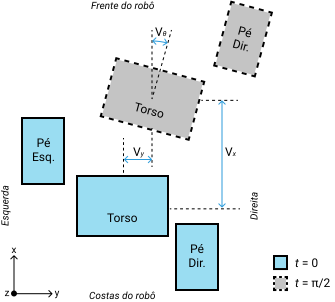
\includegraphics[scale=1]{imagens/svg/velocities-diagram}
	\caption{Diagrama da direção das velocidades da caminhada omnidirecional}
	\label{fig:math:velocities}
\end{figure}

Como mostra as equações~\ref{eq:math:velocities:intervals}, valores normalizados entre $-1.0$ e $1.0$ são utilizados para indicar as velocidades. Adotando-se $0.0$ como velocidade nula, ou sem movimento, $1.0$ como valor de velocidade máxima e $-1.0$ como valor de velocidade máxima no sentido oposto. Valores normalizados foram adotados para abstrair valores de velocidades absolutos já que futuras aplicações deste trabalho podem utilizar diferentes configurações de robôs. Desta forma, o controlador de comportamento pode abstrair a configuração do robô que está sendo controlado e enviando velocidades relativas. Adicionalmente, valores normalizados provém a integração perfeita entre as funções trigonométricas para a definição das trajetórias senoidais adotadas por \textit{Kamiri et al}.

\begin{equation}
\label{eq:math:velocities:intervals}
-1.0 \leq V_x \leq 1.0
\hspace{5mm},\hspace{5mm}
-1.0 \leq V_y \leq 1.0
\hspace{5mm},\hspace{5mm}
-1.0 \leq V_\theta \leq 1.0
\end{equation}

A cada iteração dois vetores $T$, de transferência, e $R$, de rotação, de cada pé são obtidos. Para o pé direito, utiliza-se o $t$ corrente no relógio central, já à perna esquerda um atraso de fase de $\pi/2$ é inserido.

A equação~\ref{eq:math:T_and_R:definition} mostra a definição de dos vetores $T$ e $R$. Cada um de seus elementos representam um eixo dentro deles e são gerados pelas trajetórias que são detalhadas na seção~\ref{sec:math:trajectories}.

\begin{equation}
\label{eq:math:T_and_R:definition}
T = [Foot_x,\hspace{3mm}Foot_y,\hspace{3mm}Foot_z],\hspace{5mm}R = [Foot_{roll},\hspace{3mm}Foot_{pitch},\hspace{3mm}Foot_{yaw}]
\end{equation}

Em poder desses vetores, utiliza-se os conceitos da cinemática inversa para gerar os ângulos de cada junta. Finalmente, os ângulos gerados são enviados aos motores -- como especificado na subseção~\ref{subsec:motors_abstraction} -- e, por fim, a iteração é finalizada.

\section{Orientação}
\label{sec:math:orientation}

Durante a implementação deste trabalho, nenhuma modificação foi realizada no componente de orientação originalmente desenvolvido por Kamiri \textit{et al}. Entretanto, para a implementação do cálculo da trajetórias é necessário algumas informações sobre a saída deste componente.

No final do processamento, obtém-se como saída um vetor com de aceleração linear nos eixos $x$ e $y$, como mostra a equação~\ref{eq:orientation:accel:definition}. Então, o vetor $Accel$ é utilizado para o cálculo da detecção de ``empurrões'', ou distúrbios, como visto nas equações \ref{eq:orientation:push:x} e \ref{eq:orientation:push:y}, que representação a variação na aceleração linear entre a iteração atual e a anterior.

\begin{align}
	Accel &= [Accel_x \hspace{5mm} Accel_y] \label{eq:orientation:accel:definition}
\end{align}

\begin{align}
	Push_x &= Accel[x]_t - Accel[x]_{t-1} 	 \label{eq:orientation:push:x}   \\
	Push_y &= Accel[y]_t - Accel[y]_{t-1}     \label{eq:orientation:push:y}
\end{align}

\section{Geração da trajetória}
\label{sec:math:trajectories}

Como afirmado anteriormente, a trajetória define a posição e rotação de ambos os pés de Arash durante cada momento do ciclo de caminhada, gerando como saída dois vetores $T$ e $R$, como definido na equação~\ref{eq:math:T_and_R:definition}. Kamiri \textit{et al} definem as funções que determinam cada eixo dos vetores, da equação \ref{eq:math:trajectories:foot:x} até \ref{eq:math:trajectories:foot:yaw}.

\begin{align}
      Foot_x &= \bigg(\dfrac{-cos(t) + 1}{2}\bigg) \times \bigg(\dfrac{tanh(V_x + Push_x) + H_{leg}}{\pi}\bigg)                    \label{eq:math:trajectories:foot:x}  \\
      Foot_y &= \big((-sin(t) \times B_{swing}) + (cos(t) + 1)\big) \times \bigg(\dfrac{tanh(V_y + Push_y) + H_{leg}}{2\pi}\bigg) \\
      Foot_z &= \bigg(\dfrac{sin(t)}{t + 1/2}\bigg) \times \bigg(\dfrac{tanh(V_x + V_y) \times H_{leg}}{\pi}\bigg) \\
 Foot_{roll} &= 0 \\
Foot_{pitch} &= 0 \\
  Foot_{yaw} &= \bigg(\dfrac{sin(V_\theta) + 1}{2}\bigg) \times \bigg(\dfrac{-cos(t) + 1}{2} \times V_\theta\bigg)     \label{eq:math:trajectories:foot:yaw}
\end{align}

Onde $t$ representa o tempo atual normalizado em cada ciclo; $B_{swing}$ representa a quantidade de compensação de balanço lateral que o corpo deve efetuar para compensar a dinâmica do movimento das pernas; $Push$ -- definido na seção~\ref{sec:math:orientation} -- é a quantidade de distúrbio causado por desvios na trajetória; por fim, $H_{leg}$ é o valor do tamanho da perna, extraído da estrutura do robô.

Nota-se que as funções $Foot_{roll}$ e $Foot_{pitch}$ são definidas como $0$ pois, em resultados experimentais, os efeitos durante a caminhada mostraram-se desprezíveis \cite{karimionline}.

\section{Cinemática Inversa}

Descobrir a posição de um parte do robô a partir dos ângulos de suas juntas, \textit{forward kinematics}, é uma tarefa fácil e pode ser realizada eficientemente. Porém, o oposto -- dado um ponto e calcular os ângulos das juntas que o alcancem; processo conhecido como \abrv[IK -- conhecido como \textit{Inverse Kinematics}, ou cinemática inversa]{IK (do inglês \textit{inverse kinematics} ou cinemática inversa)}-- não é uma tarefa tão simples.

Enquanto a problemas envolvendo a \textit{forward kinematics} possuem uma solução única, na \textit{IK} podem haver múltiplas soluções ou nenhuma \cite{spong2005robot}. Pode-se observar este fato ao tocar a ponta do próprio nariz, já que existem diversas combinações de posições do ombro, cotovelo, pulso e falanges que resolvem este problema; Entretando, usando as configurações de braço de um Tiranossauro o problema não teria solução, uma vez que o braço é demasiado curto para efetuar tal tarefa.

Aplicando a teoria da cinemática inversa ao problema proposto, Kamiri \textit{et al} apresenta uma solução direta aproveitando-se das limitações impostas pela configuração das juntas de Arash.

\begin{equation}
	\label{eq:math:ik:P:definition}
	P = [Hip_{yaw}, Hip_{roll}, Hip_{pitch}, Knee, Foot_{pitch}, Foot_{roll}] = iK(T, R)
\end{equation}

Na equação~\ref{eq:math:ik:P:definition}, vemos a definição do vetor P que mantém os valores dos ângulos de todas as juntas. Ele é a saída da função $iK$ que recebe como parâmetros os vetores $T$ e $R$ já definidos na equação~\ref{eq:math:T_and_R:definition}.

O processo de formulação das equações inicia-se a partir do nó principal do quadril descendo para o fim da cadeia, nos pés; onde encontra-se o fim da cadéia e o ponto de destino.

Na primeira etapa, a figura~\ref{fig:ik:upperview} mostra uma tomada de cima de Arash auxiliando na visualização da equação \ref{eq:ik:upper:hip:yaw}. Nota-se que, embora os pés de Arash não possuam rotação no eixo $yaw$ (figura~\ref{fig:architecture:arash:actuators_orientations}) a rotação $yaw$ aplicada no quadril, afeta toda a cadeia.

\begin{figure}[htb]
	\centering
	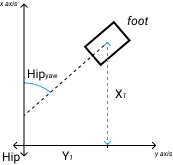
\includegraphics[scale=1.5]{imagens/svg/inverse-kinematics-upperview}
	\caption{Diagrama da visão superior da estrutura de Arash que representa da equação~\ref{eq:ik:upper:hip:yaw} até~\ref{eq:ik:upper:z:2}}
	\caption*{\cite{karimionline}}
	\label{fig:ik:upperview}
\end{figure}

\begin{align}
	P[Hip_{yaw}] &= R_{yaw}                             \label{eq:ik:upper:hip:yaw}  \\
	         X_2 &= T_x cos(R_{yaw}) + T_y sin(R_{yaw})  \label{eq:ik:upper:x:2}      \\
	         Y_2 &= -T_x sin(R_{yaw}) + T_ycos(R_{yaw})   \label{eq:ik:upper:y:2}      \\
	         Z_2 &= T_z                                    \label{eq:ik:upper:z:2}
\end{align}

Seguindo o processo de parametrização dos ângulos das juntas, observa-se na figura~\ref{fig:ik:frontalview} a visão frontal de Arash provendo uma visualização geométrica das equações~\ref{eq:ik:p:hip:roll} até \ref{eq:ik:z:3}. Nesta figura observa-se, também, o movimento no eixo $roll$ do quadril sendo compensado pelo movimento no sentido oposto (mas no mesmo eixo) do pé, afim de compensar o alinhamento do pé com o piso.

\begin{figure}[htb]
	\centering
	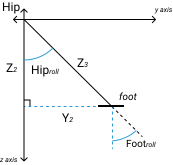
\includegraphics[scale=1.5]{imagens/svg/inverse-kinematics-frontalview}
	\caption{Diagrama da visão frontal de Arash que representa da equação~\ref{eq:ik:p:hip:roll} até~\ref{eq:ik:z:3}}
	\caption*{\cite{karimionline}}
	\label{fig:ik:frontalview}
\end{figure}

\begin{align}
	 P[Hip_{roll}] &= atan\bigg(\dfrac{Y_2}{Z_2}\bigg)                    \label{eq:ik:p:hip:roll}     \\
	P[Foot_{roll}] &= -P[Hip_{roll}] + R_{roll}                            \label{eq:ik:p:foot:roll}    \\
			   X_3 &= X_2                                                   \label{eq:ik:x:3}            \\
			   Y_3 &= Y_2                                                    \label{eq:ik:y:3}            \\
	           Z_3 &= \sqrt{Y_2^{\hspace{1mm}2} + {Z_2}^{\hspace{1mm}2}}      \label{eq:ik:z:3}
\end{align}

Na terceira etapa, a figura~\ref{fig:ik:frontalview} mostra a visão frontal de Arash, também, provendo uma visualização geométrica das equações~\ref{eq:ik:p:hip:roll} até \ref{eq:ik:z:3}.

\begin{figure}[htb]
	\centering
	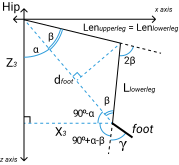
\includegraphics[scale=1.5]{imagens/svg/inverse-kinematics-sideview}
	\caption{Diagrama da visão lateral de Arash que representa da equação~\ref{eq:ik:p:hip:roll} até~\ref{eq:ik:z:3}}
	\caption*{\cite{karimionline}}
	\label{fig:ik:sideview}
\end{figure}

\begin{align}
	       d_{foot} &= \sqrt{Z_3^{\hspace{1mm}2} + X_3^{\hspace{1mm}2}}     \label{eq:ik:d:foot}        \\
	         \alpha &= atan\bigg(\dfrac{X_3}{Z_3}\bigg)                      \label{eq:ik:alpha}         \\
	          \beta &= acos\bigg(\dfrac{d_{foot}}{2 \times Leg_{len}}\bigg)   \label{eq:ik:beta}          \\
	 P[Hip_{pitch}] &= \alpha + \beta                                          \label{eq:ik:p:hip:pitch}   \\
	        P[Knee] &= -2 \beta                                                 \label{eq:ik:p:knee}        \\
	P[Foot_{pitch}] &= \gamma = -\alpha + \beta + R_{pitch}                      \label{eq:ik:p:foot:pitch}
\end{align}

Adicionalmente, a cada junta é somado um parâmetro de deslocamento -- não incluso nas equações de \textit{IK} --, também conhecido como \textit{offset}, para compensar possíveis erros provenientes de desalinhamentos no momento de montagem do robô, ou folgas nas engrenagens dos atuadores.

Finalmente, com as equações de \textit{IK} definidas, o \textit{walking gait}, com o auxílio dos componentes de orientação e \textit{proxy}, é apto a fazer os cálculos necessários para determinar os movimentos de caminhada.

	
	% Capitulo 4: Quarto cap���tulo (arquivo Includes/Capitulo4.tex)
	% Capítulo 4
\chapter{Projeto e implementação do \textit{Walking gait}}
\label{ch:Math}

\begin{guide}
	Detalhar implementação do walking gait
\end{guide}

\begin{guide}
	Detalhar matemática dos movimentos.
\end{guide}

\section{\textit{Walking gait}}

Nesta seção detalhes arquiteturais da implementação do \textit{walking gait} serão descritos.

O \textit{walking gait} é o componente que coordena a caminhada mantendo o estado drobô, sabendo onde cada perna encontra-se e o seu estágio durante a caminhada. Desta forma, quando algum evento de perturbação, ou de ajuste, é disparado o \textit{walking gait} inicia a atualização das juntas a partir do estado atual. Assim, podemos descrever a caminhada como um evento contínuo no tempo.

Para realizar a tarefa de forma adequada, o componente faz uso de multi-processamento. Três \textit{threads} dentro do componente são responsáveis por tarefas específicas essenciais ao complemento do comportamento geral da caminhada: A \textit{thread} de rede, a \textit{thread} atualização dos motores e a \textit{thread} principal.

\subsection{\textit{Thread} principal: Da geração da trajetória até a aplicação às juntas}

\begin{figure}[h!]
	\centering
	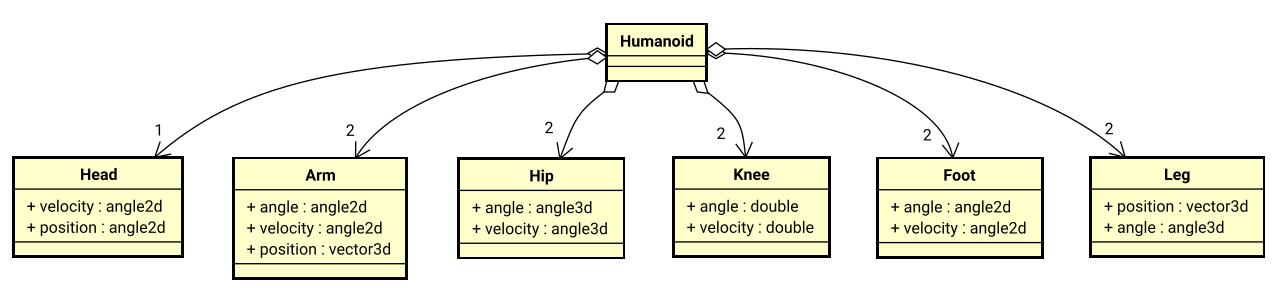
\includegraphics[scale=0.4]{imagens/svg/walkinggait-domain}
	\caption{Diagrama de domínio do \textit{walking gait}.}
	\label{fig:walkinggait:domain}
\end{figure}

A figura~\ref{fig:walkinggait:domain} mostra o diagrama de domínio das classes relevantes aos dados que o componente manipula. Nela podemos ver a classe $Humanoid$ é uma agregação de diversas outras classes que representam cada parte de Arash. É possível também observar que nas classes $Head$, $Arm$, $Hip$, $Knee$, $Foot$ existem dados ângulo e velocidade. Isso se dá por causa que componente utiliza essas informações para calcular o próximo estado do sistema em caso de algum distúrbio. Nota-se também, que a classe $Leg$ aparece de forma ambígua, já que existem as definições de $Hip$, $Knee$ e $Foot$. Porém, a classe $Leg$, representa os dados da cinemática inversa de uma perna, enquanto as demais classes guardam o estado atual das partes que representam.

Nota-se, também, a notação dos dados utilizados: $angle2d$, $angle3d$ e $vector3d$. Note que todos os tipos possuem o sufixo numérico, que indica a quantidade de dimensões aquela classe guarda, e a letra, que indica o tipo de seus dados, no caso $d$ que significa $double$. Para ângulos, $2$ dimensões significa que as dimensões $pitch$ e $roll$ são guardadas; já para $3$ dimensões as orientações $roll$, $pitch$ e $yaw$ são guardadas. Para vetores, os valores $x$, $y$ e $z$ são guardados.



\subsection{Servidor de controle}

A \textit{thread} de rede roda um servidor \textit{UDP} que aceita objetos serializandos em \textit{JSON} contendo informações de controle.




\section{Seção 1}
\label{sec:Orientacao}

Teste para símbolo

\simb[$\lambda$ (algum símbolo)]{$\lambda$}


\section{Seção 2}

Teste para abreviatura 

\abrv[IFRN -- Instituto Federal do Rio Grande do Norte]{IFRN}

\abrv[DIATINF -- Diretoria Acadêmica de Gestão e Tecnologia da
Informação]{DIATINF}

	
	% Capitulo 5: Quinto cap���tulo (arquivo Includes/Capitulo5.tex)
	% Cap�tulo 5
\chapter{Capítulo 5}

\guide{Detalhar implementação, integração e simulação e testes.}

\section{Seção 1}

\guide{Detalhar implementação.}

\section{Seção 2}

\guide{Detalhar simulação.}

\section{Seção 3}

\guide{Detalhar simulação.}


Seção 3
		
	% Consideracoes finais
	\chapter{Conclusão}

Este trabalho apresentou o processo de implementação do \textit{walking gait} do time AUTUofM, descrevendo as soluções de software e justificando as decisões tomadas. Apresentou-se a abordagem tomada para mover a implementação da placa microcontroladora \textit{OpenCM9.04} para um \textit{software} dentro do controlador principal.

Para tanto, foram realizadas modificações no \textit{firmware} da \textit{OpenCM9.04} criando um componente \textit{Proxy} que encaminha os comandos recebidos através da porta \textit{USB} aos motores. Comandos estes gerados pela nova implementação do \textit{walking gait}, desta vez utilizando a linguagem C++. O mesmo método usando um padrão de trajetórias senoidais e recuperação de distúrbios proposto por Karimi \textit{et al} foi utilizado para a nova implementação.

\begin{figure}[htb]
	\centering
	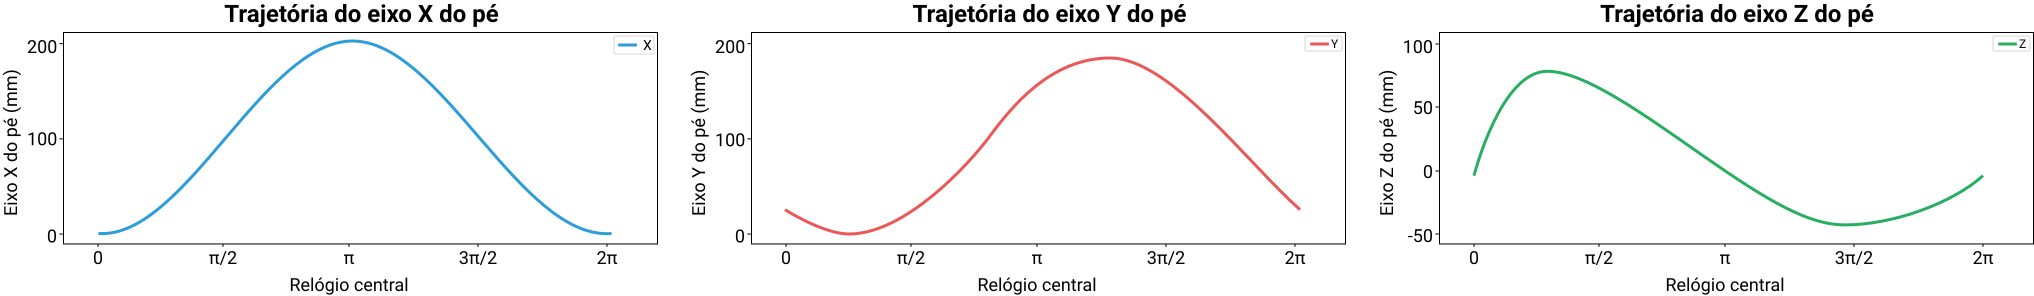
\includegraphics[width=\textwidth]{imagens/svg/conclusion-trajectories-graph}
	\caption{Gráficos das trajetórias do ciclo de caminhada nos eixos X, Y e Z gerados pela nova implementação do \textit{walking gait}.}
	\label{fig:conclusion:trajectories:graph}
\end{figure}

\begin{figure}[htb]
	\centering
	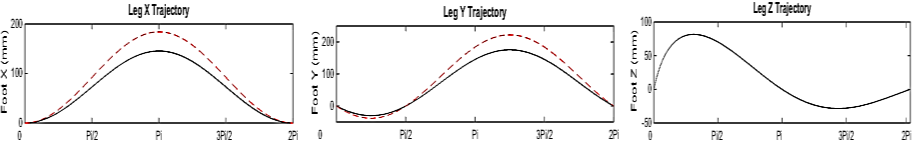
\includegraphics[width=\textwidth]{imagens/conclusion-trajectories-graph-old}
	\caption{Gráficos das trajetórias do ciclo de caminhada nos eixos X, Y e Z gerados Karimi \textit{et al}.}
	\label{fig:conclusion:trajectories:graph:old}
\end{figure}

Devido a falta de dados concretos sobre a geração das trajetórias, foram utilizadas comparações visuais com os gráficos fornecidos por Karimi \textit{et al} em seu trabalho. Nas figuras \ref{fig:conclusion:trajectories:graph} e \ref{fig:conclusion:trajectories:graph:old} é possível observar, respectivamente, os gráficos das trajetórias geradas pelo novo e pelo velho \textit{walking gait}. Em ambas as imagens possível observar a trajetória nos eixos $X$, $Y$ e $Z$ separados. No eixo vertical do gráfico o trajetória é escalada em milímetros. No eixo horizontal a escala é no ciclo do relógio central.

Ainda na figura~\ref{fig:conclusion:trajectories:graph:old} observa-se uma linha vermelha pontilhada, que indica a compensação realizada pelo sistema durante um evento de distúrbio realizado no robô físico \cite{karimionline}. Tal evento não foi possível de ser reproduzido pela falta de acesso ao robô físico.

Em relação ao movimento da caminhada, foi possível validar a geração da cinemática inversa através das animações, em tempo real, produzidas pelo visualizador 3D. A figura~\ref{fig:conclusion:arash:frames} observa-se 4 \textit{capturas de tela} do visualizador em uma caminhada com $V_x = 0.5$ da perspectiva lateral, na primeira linha, e pela perspectiva frontal na segunda linha. Nas primeira coluna, $t = 0$, observa-se o mostra uma posição estável, com ambos os pés no chão. Na segunda, observa-se o momento em que o pé direito é levantado, onde $t = \pi/2$. A terceira coluna mostra o momento em que $t = \pi$, metade do ciclo, em que ambos os pés voltam a tocar no chão. Então, a quarta coluna mostra o momento em que o pé esquerdo sai do chão, $t = 3\pi/2$. Seguindo o ciclo, o relógio é reiniciado e o estado retorna ao da primeira coluna.

\begin{figure}[htb]
	\centering
	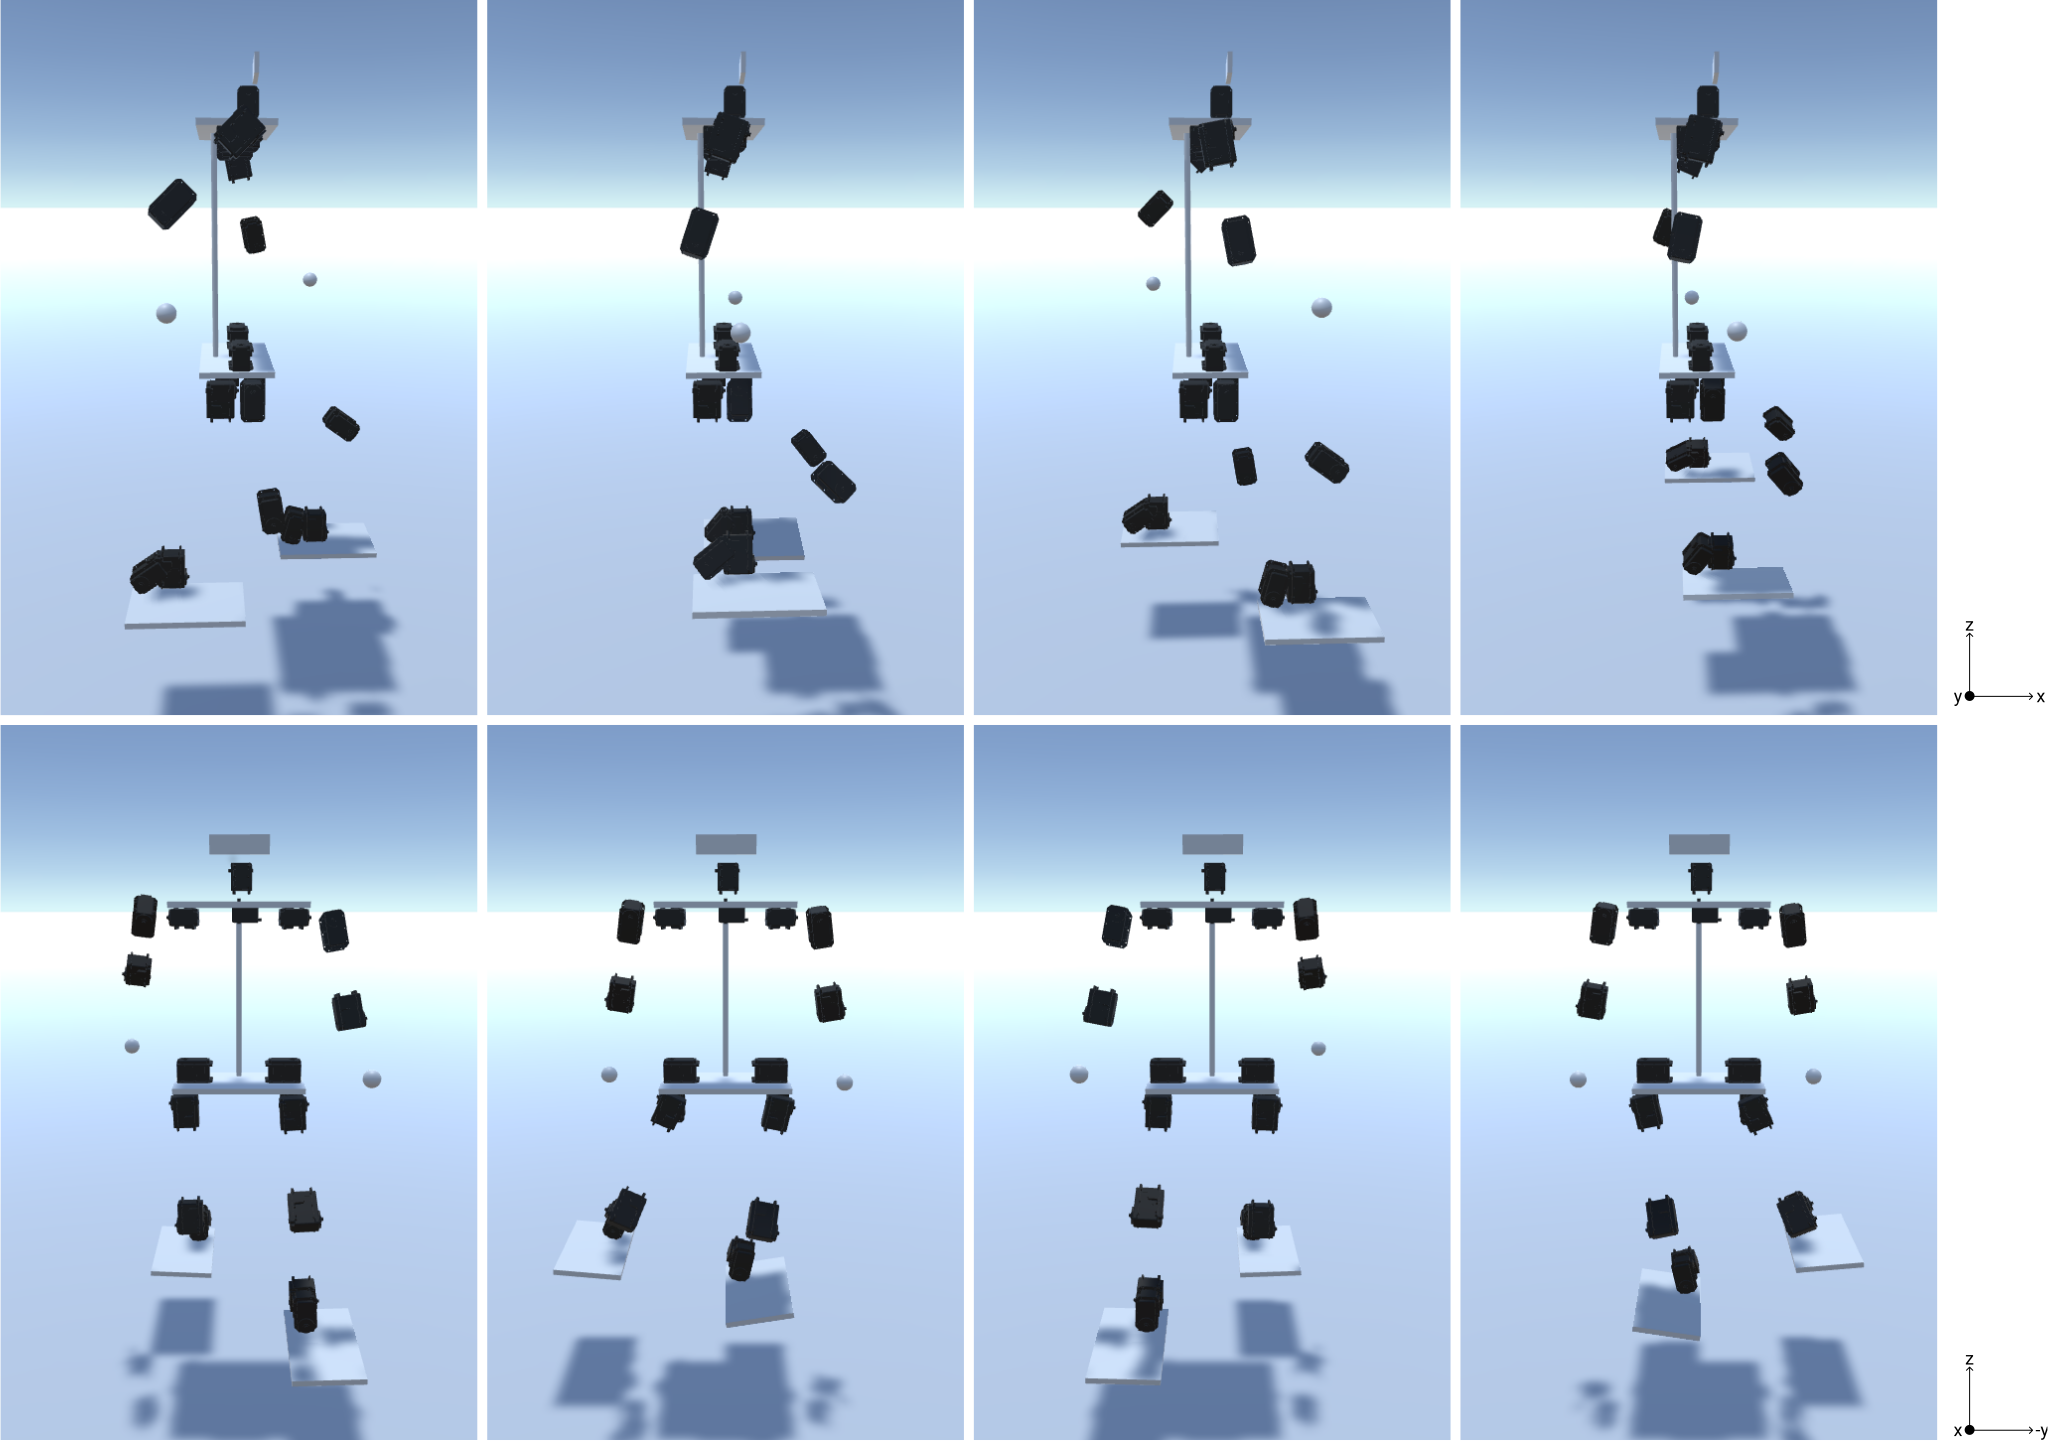
\includegraphics[width=\textwidth]{imagens/svg/conclusion-arash-frames}
	\caption{Visualização frontal e lateral dos movimentos da caminhada.}
	\label{fig:conclusion:arash:frames}
\end{figure}

Um esquema de configurações persistidas em disco em arquivos JSON atacou diretamente o problema da falta de controle sobre as configurações geradas. Assim, os arquivos de configuração podem ser versionados utilizando algum sistema de versionamento de código.

Apesar da simulação não ter sido implementada neste trabalho, seu futuro acomplamento será menos complexo, já que a nova implementação usa o conceito de um sistema distribuído baseado em serviços.

Considerando que o \textit{walking gait} funciona dentro do controlador principal. Futuras melhorias que possam exigir mais recursos -- processamento ou memórias RAM e ROM -- podem ser implementadas.

Finalmente, de acordo com os resultados obtidos, podemos concluir que a implementação do \textit{walking gait} foi realizada alcançando solucionando os problemas listados neste trabalho. Adicionalmente, o resultado pode ser utilizado como base para diversas melhorias descritas na seção~\ref{sec:conclusion:future}.

\section{Trabalhos futuros}
\label{sec:conclusion:future}

As atualizações realizadas no \textit{walking gait} original do time AUTUofM agora permitem diversas expensões no código para futuras atualizações e investigações. Assim, os próximos parágrafos descrevem alguns possíveis trabalhos futuros.

Este trabalho foi todo desenvolvido apenas usando \textit{software} e visualização 3D dos ângulos gerados. A implementação e teste usando o robô real é um passo fundamental para a consolidação deste trabalho.

A implementação sem a utilização de um sistema de simulação apropriado não garante que o robô realmente possa caminhar. O uso do visualizador 3D mostra um esboço do movimento, sem a real caminhada, que pode gerar novos desafios. Em paralelo, embora os dados do leitor de orientação sejam levados em conta tem todos os cálculos, seus efeitos não foram testados. Consequentemente, a integração do módulo do \textit{walking gait} a um \textit{framework} de simulação é um passo em direção a um sistema mais completo.

Segundo, durante uma tarefa genérica realizada por um robô não apenas se caminha. Movimentos como chutes, levantar-se do chão, pegar um copo -- entre outros -- são normalmente pré-gravados na etapa de desenvolvimento e durante a tarefa são apenas reproduzidos. Desta forma, um módulo para gravar e reproduzir estes movimentos faz-se necessário.

Terceiro, o fato do \textit{walking gait} rodar fora da \textit{OpenCM9.04} adiciona algum atraso extra entre o cálculo dos ângulos e a aplicação aos motores. Adicionalmente, os dados processados do leitor de orientação demoram mais a ter efeito nos cálculos das correções. Porém, o seu impacto real, durante a caminhada, não pode ser explorado neste trabalho deixando esta investigação para trabalhos futuros.

Quarto, alguns métodos de caminhada utilizam sensores nos pés de forma a detectar quando há o contato com o chão. Este momento é crítico pois, em caso de algum distúrbio, se houver uma diferença do momento esperado para o momento real do toque, ações diferenciadas poderão ser tomadas. Com isto em mente, sabe-se que os motores da série \textit{MX} possuem \textit{feedback} de carga baseado na voltagem de saída interna, onde deverá ser possível medir a diferença nas cargas esperadas e reais afim de prever se o pé está em contato com o chão.

Finalmente, outros métodos mais complexos de caminhada, utilizando mais processamento e mais memória, poderão ser implementados já que a barreira de recursos do \textit{OpenCM9.04} foi quebrada. 
	
	% Bibliografia (arquivo Capitulos/Referencias.bib)
	\bibliography{capitulos/Referencias}
	\bibliographystyle{abnt-alf}
	
	% Ap���ndice A (arquivo Includes/ApendiceA)
	% Ap�ndice
\apendice
\chapter{Primeiro apêndice}

Os apêndices são textos ou documentos elaborados pelo autor, a fim de
complementar sua argumentação, sem prejuízo da unidade nuclear do trabalho.

	
	% Anexo A (arquivo Includes/AnexoA)
	% Anexo
\anexo
\chapter{Primeiro anexo}

Os anexos são textos ou documentos não elaborado pelo autor, que servem de
fundamentação, comprovação e ilustração.

	
	% P���gina em branco
	\newpage

\end{document}